\documentclass[12pt]{article}

\usepackage{fullpage}
\usepackage{graphicx, rotating, booktabs} 
\usepackage{times} 
\usepackage{natbib} 
\usepackage{indentfirst} 
\usepackage{setspace}
\usepackage{grffile} 
\usepackage{hyperref}
\usepackage{adjustbox}
\setcitestyle{aysep{}}


\singlespace
\title{\textbf{Summary of Previous Empirical Work on the Arms-Alliances Tradeoff}}
\author{Joshua Alley\footnote{Graduate Student,
Department of Political Science, Texas A\&M University.}}
\date{{\normalsize \today}}

\bibliographystyle{apsr}

\begin{document}

\maketitle 


\section*{Introduction}

What do we know about the association between arms and alliances? Domestic military spending and international alliances are two of the most important policies in international security. While most scholars examine arms or alliances in isolation, others address how states mix these two policies in pursuit of security. 

To assess the state of research on the arms-alliances tradeoff, I undertook a comprehensive literature review. The review cataloged the primary claim, theory, research design, and evidence of 26 papers.\footnote{In the interest of parsimony and time, I did not comprehensively summarize work on free-riding in NATO, which is a literature unto itself. Instead, I focused on the papers that made major methodological or theoretical innovations.} I was interested in how each study contributed to our understanding of the general relationship between arms and alliances. 

Our knowledge of the arms-alliances tradeoff is incomplete at best. There are two competing theoretical camps--- one sees arms and allies as substitutes, while the other argues that these policies are complements. Theories of arms and alliances as complements do a poor job developing mechanisms to support their claim. Even with these theoretical issues, it is hard to assess the balance of knowledge because of serious empirical problems. 

Few studies generate a credible estimate of the association between arms and alliances. Many scholars test general claims with limited samples and misspecified models. Due to poor empirical design in many studies, it is difficult to identify meaningful patterns in the results. 

The most trustworthy models suggest that any association between arms and alliances is conditional. The best general model of the arms-alliances tradeoff only finds substitution in a particular type of alliances. Mixed results from studies of specific alliances underline this conclusion. 

Current theories of the arms-alliances tradeoff do not make conditional claims, however. Instead, researchers make exclusive claims that arms and allies are substitutes or complements. I start this paper by summarizing the theoretical logic underlying each paradigm. Then, I assess the research designs that tested those theoretical claims. The last section concludes by discussing open issues in the arms-alliances tradeoff literature and considerations for future research. 


\section*{Arms and Allies as Substitutes}

If arms and alliances are substitutes, then additional alliances or capability from alliance partners should lead to decreases in domestic military spending.\footnote{All empirical tests focus on this prediction, although substitution logic also predicts that when alliances become more costly, states will turn to domestic arms.} Two distinct theories expect this inverse association between alliances and domestic arms. Substitution theories of the arms-alliances tradeoff and the economic theory of alliances focus on how arms and allies both produce security, leading states to replace domestic military spending with allied spending. 

Both theories use the opportunity costs of military spending to motivate substitution. Although military spending can have positive economic and technological spinoffs \citep{DegerSen1995, WhittenWilliams2011}, allocating funds to the military takes resources away from other social and economic policies. Leaders can use these other public and private goods to ensure their political survival \citep{BDMetal2002}. Therefore if states can rely on their allies to provide security, they have ample domestic political motives to reduce spending. 

Predictions of substitution between arms and alliances rely on the insight that states can use multiple policies means to achieve their foreign policy goals \citep{MostStarr1989}. \citet{Morrow1993} argues that domestic arms and alliances are both sources of military capability, allowing states to substitute between the two in their search for security. Instead of internal balancing through spending more on domestic arms, states can rely on external balancing through allied capability \citep{Conybeare1992}. 

The marginal costs of arms and alliances determine which policy states use to increase their security \citep{Sorokin1994}. For instance, some evidence suggests that as the opportunity cost of military spending increases, states are more likely to form alliances \citep{Kimball2010, AllenDigiuseppe2013}. Measuring the foreign policy costs of a potential alliance has proved more difficult, and is the main barrier to examining whether higher costs of an alliance lead states to rely more on military spending. These differences in the type of costs associated with each policy means that arms and alliances are not perfect replacements for one another. 

Arms and allies are imperfect substitutes. States can rely on their own arms in any contingency, but domestic military capabilities take a long time to develop. Because members have divergent foreign policy interests, alliances are a less reliable source of capability than domestic arms, but provide immediate capability gains. The moment a treaty enters into force, alliance members gain their partner's support.

As an alliance becomes more reliable, that treaty becomes more like domestic arms as a source of capability. Therefore, more credible alliance treaties are a better substitute for domestic arms. \citet{DigiuseppePoast2016} expand on this insight by arguing that because defense pacts with a democracy are more credible, these alliances will lead to reductions in spending. 

The theoretical logic of substitution theory is clear, but we have little evidence for these claims. Only four studies test substitution of alliances for arms using military spending or personnel as the dependent variable. This lack of attention reflects more emphasis on possible free riding in alliances. 

The economic theory of alliances also predicts that alliances lead to reduced domestic arms, but relies on a different mechanism. \citet{OlsonZeckhauser1966} treat security from an alliance as a public good, which generates a collective action problem for members. Each members military spending is a contribution to the public good, but all members have incentives to free ride on the effort of their partners. As a result, they predict that larger members of an alliance will bear a higher defense burden, because these states have a higher absolute value of the public good. Olson and Zeckhauser interpret a positive correlation between GDP and the ratio of defense spending to GDP as evidence of free-riding. Under this theory, alliance membership leads small states to reduce defense spending. 

Olson and Zeckhauser's claims sparked extensive debate about free riding by alliance members. Much of the discussion focused on NATO, but other scholars checked the correlation between defense burdens and GDP in other alliances, with mixed results \citep{Reisinger1983, Thies1987, GatesTerasawa1992, OnealWhatley1996, Siroky2012}. The best evidence of free-riding is \citet{PluemperNeumayer2015}, who show that many NATO allies are unresponsive or even reduce spending when growth in Soviet spending exceeds growth in US spending, and that the degree of free-riding depends on distance from the USSR. As with substitution theories, free-riding may only occur when treaty commitments are sufficiently credible \citep{GatesTerasawa1992}. 

A theoretical extension of the economic theory of alliances conceptualizes military spending as having public and private benefits \citep{ConybeareSandler1990}. These joint product models lead to different predictions, because as the ratio of private to public benefits increases, we should observe less free-riding \citep{Murdoch1995, SandlerHartley2001}. Other studies divided types of military spending according to the benefit they provide, especially nuclear and non-nuclear defense effort \citep{Hansenetal1990}. Nuclear arms provide a pure public good through deterrence, while conventional spending has private benefits such as increased border security. 

Emphasizing free riding creates several issues for the economic theory of alliances. First, the concept of free-riding itself is problematic. Reductions in spending by NATO members could reflect decreased threat perceptions or a bargain with the United States \citep{Lanoszka2015}. Distinguishing between free-riding and exchange is difficult, especially if smaller alliance members trade security for autonomy in asymmetric alliances \citep{Morrow1991}. 

Emphasizing free riding limits the applicability of evidence from the economic theory of alliances to a general understanding of the arms-alliances tradeoff. The standard dependent variable is the defense burden--- military spending as a share of GDP. It is difficult to identify a model of this ratio dependent variable, casting serious doubt on many of the studies that rely on correlations or rank orderings of defense burdens and economic size for evidence \citep{PluemperNeumayer2015}. 

Despite problems from the focus on free-riding in the economic theory of alliances, substitution theories of alliances have a clear internal logic and mechanism. This theoretical clarity allowed scholars to set general expectations about the relationship between arms and alliances--- substitution theory is the best known theoretical paradigm in the arms-alliances tradeoff literature. Policymakers complaints about free-riding further reinforced the perception that alliances lead to reduced defense effort by junior partners. While popular, substitution theory is incomplete.

The major weakness of substitution theories is their emphasis on security as the only output of an alliance. Substitution theory acknowledges that multiple policies can advance a particular goal, but it does not acknowledge multiple foreign policy goals. Therefore, this perspective cannot capture the full range of how alliances may affect domestic arms. 

States have a range of foreign policy goals. Even security focused paradigms like neorealism admit states may have different preferences over whether to maintain or change the status quo \citep{Schweller1994, Walt2009}. Substitution theory addresses some of the domestic political incentives states face in making security policy, but it provides little detail about possible differences in foreign policy. By contrast, theories of arms and alliances as complements have a less clear internal logic, but consider diverse foreign policy aims. 


\section*{Arms and Allies as Complements}

The literature on arms and alliances as complements is less developed. These theories expect that arms and alliances are positively correlated--- states that form an alliance will increase military spending. Scholars have proposed several explanations for this prediction.

\citet{Diehl1994} argues that arms and alliances are not comparable policies and have multiple purposes besides deterrence, so substitution is unlikely. He then lists several mechanisms that might generate complementarity between arms and alliances, but is not clear about which is most important. These mechanisms include the possibility that alliances require increased foreign policy activity, or that major powers increase military spending to cover free-riding by junior alliance partners. The most general argument asserts that autonomy benefits from an alliance increase the marginal value of military spending.

\citet{MorganPalmer2006} also use an increase in the value of military spending to motivate complementarity in their study of how states use different foreign policy instruments. Their theory starts with the premise that states have two foreign policy goals--- maintenance and change. States then allocate all their foreign policy resources to pursue a mix of maintenance and change across a range of issues. Due to budget constraints, there is a tradeoff between maintenance and change. To examine substitution between different foreign policy instruments, they start with the assumption that states choose the most efficient policy tool to realize their goals. 

Given this assumption, there are three reasons states might increase their use of a particular policy. The first is an increase the overall resources available to the state, and the second is changes in relative preferences for maintenance and change. The last path is changes in the efficiency of different policies, which is the only path that leads to substitution. In this model, substitution is motivated by states moving resources from less to more efficient policies, which they argue is uncommon. 

Rather, Morgan and Palmer argue that alliances increase the amount of resources available to the state, which frees up resources that can then be dedicated to pursuing other goals. Alliances expand the foreign policy possibilities for a state, which makes them more likely to increase military spending. As an illustrative example, they argue that an alliance with the US gave Britain and France extra resources to pursue change in the Middle East during the 1957 Suez crisis.  

By only examining foreign policy tradeoffs, Morgan and Palmer ignore domestic incentives to reduce military spending. Because states do not expend the same kinds of resources on domestic arms and alliances, the concept of a foreign policy ``budget'' is nebulous. These weaknesses aside, Morgan and Palmer make a valuable contribution by distinguishing between goals of maintenance and change, and possible tradeoffs between the two.

Neither Diehl nor Morgan and Palmer adequately explain the process by which joining an alliance increases military spending. But if arms and allies are imperfect substitutes as Diehl argues, then these two policies also have some characteristics that allow for substitution. Greater clarity about the mechanism by which alliances increase the marginal benefits of military spending is necessary. 

Another mechanism behind complementarity is cooperation and policy coordination between alliance members. \citet{Palmer1990} conceptualizes relations among alliance members as an iterated prisoner's dilemma, where states can communicate and use side issues to overcome collective action problems. \citet{QuirozFlores2011} attributes a positive spatial correlation in the defense burden of allied states to increased cooperation between allies.

The cooperation thesis acknowledges collective action problems in the economic theory of alliances, but argues that these problems can be overcome. There is some evidence that alliances facilitate cooperation in other issue areas \citep{Gowa1995, GowaMansfield2004, Poast2012, Poast2013}. Cooperation on side issues will not necessarily lead to increases in spending as states overcome collective action problems. Small states can use concessions in other issue areas as part of a bargain with their patron that allows for reduced military spending. Intra-alliance cooperation is an insufficient explanation of complementarity between arms and allies. 

The challenge for complementarity theory is clear--- scholars must develop better theoretical explanations for their prediction that alliance membership leads to increases in military spending. Neither general arguments or the cooperation thesis provide a sufficient explanation for possible complementarity. The shortcomings of current theories do not imply that scholars should rule out complementarity between arms and alliances, however. Theories of arms and allies as complements still make a valuable contribution to knowledge of the arms alliances tradeoff, by considering diverse foreign policy goals. 


\section*{The State of Arms-Allies Theory}

Given arguments that arms and alliances are complements or substitutes, what is the overall theoretical development of the literature? Work on arms and alliances is characterized by two disjointed perspectives with distinct strengths and weaknesses. Debate over whether arms and allies are substitutes or complements treats the two perspectives as incompatible. Framing substitutes and complements as competing hypotheses has stunted theoretical progress, as neither perspective incorporates the key insight of the other. 

Substitution theories have not engaged with the claim that states have diverse foreign policy goals. Complementarity theories do not consider domestic political incentives for security-seeking states to rely on allied capability. A general theory of the arms-alliances tradeoff must incorporate both of these elements--- domestic political incentives to substitute and diverse foreign policy goals. 

Because the strengths and weaknesses of complementarity and substitution theories mirror each other, it may be possible to combine the two. Rather than pitting the two perspectives against each other, a more fruitful approach should consider whether each applies in different circumstances. This combination implies a conditional association between arms and alliances. 

\citet{DigiuseppePoast2016}'s argument that substitution hinges on the credibility of an alliance treaty is a useful first step. By acknowledging heterogeneous effects of alliances, the theory and results suggest that arms and alliances are not uniformly substitutes or complements. The main shortcoming of this work is that while it acknowledges findings of a positive correlation between arms and alliances, it does not address those cases. 

DiGiuseppe and Poast employed two theoretical mechanisms from democratic credibility and substitution theory. Explaining when arms and allies are complements will require more effort. But complementarity and substitution theories share a common element that can facilitate theoretical progress. 

Both substitution and complementarity theories use an income effect to connect a state's alliance portfolio to changes in military spending. Income effects address how an actor changes its consumption basket after an increase in its budget.\footnote{For example, rising income usually leads individuals to add more protein to their diet.} Both theories predict that gains from an alliance will change how states utilize other resources. The difference between the two paradigms is that they focus on changes in the consumption of different goods. Substitution theory focuses on shifts in domestic consumption, while complementarity theories consider changes in foreign policy. 

Therefore, the key task for scholars is articulating when states will emphasize domestic or international gains. Whether an alliance produces security or autonomy \citep{Morrow1991}, is essential to understanding how states use the capability gains from a treaty. Security reflects interests in maintaining the status quo, while autonomy is the ability of states to seek changes in the status quo. Security-producing alliances will facilitate domestic gains, while autonomy-generating alliances will lead to foreign policy gains. 

A degree of security is a necessity for all states, as it allows them to set other policies as they see fit \citep{Lake1996}. Under substitution, additional allied capability causes a state to shift its domestic consumption away from providing security towards other economic and social goods that are otherwise luxuries. In complementarity theories, an alliance expands what a state can achieve in its foreign policy, so states can consume additional foreign policy goods. 

Contextual factors may also alter the nature of the arms-alliances tradeoff. Between nuclear weapons, changing norms about international conquest \citep{Fazal2011}, economic interdependence \citep{Frieden2006}, and changes in the cost/complexity of weapons systems \citep{Bitzinger2003} the international environment has changed in dramatic ways, especially after 1945. So far, no theories of the arms-alliances tradeoff have addressed whether these shifts in the international environment alter states' goals. Constraints on how much change or autonomy a state can achieve in foreign policy may lead to more emphasis on domestic gains from alliances.   

Regardless of how theories of the arms-allies tradeoff evolve, clear hypotheses are indispensable. Without precise theoretical predictions, the risk of spurious results from poor research designs increases. Most current theories do not specify all the possible observable implications, or do not clarify the appropriate dependent variable. This lack of clarity is reflect in poor research designs. Another issue with predictions from current theories is their inadequate attention to possible scope conditions. 

The most salient example of a problem with scope conditions is the debate over free-riding in alliances. Most scholars ignore possible differences between major and non-major powers. The economic theory of alliances expects greater free riding by smaller alliance members, but many tests of this theory examine alliances between major powers \citep{Thies1987, ConybeareSandler1990, Siroky2012}. 

If smaller states are more likely to use alliances as a source of security, rather than to increase their foreign policy autonomy \citep{Morrow1991}, then autonomy-seeking major powers have less incentive to substitute alliances for arms. Other theories beyond the economic theory of alliances must consider these differences between major and minor powers. If the relationship between arms and allies is fundamentally different for major powers, studies of major power alliances will only tell part of the story.  


The theoretical and empirical importance of scope conditions points to the other major problem in scholarship on the arms-alliances tradeoff--- many early empirical results have limited viability. Absent reliable empirical results, assessing the relative value of different theories is impossible. Despite the general claims in different theories, most studies of the arms-allies tradeoff provide poor evidence for their claims. Many researchers use limited samples of states or alliances, or fail to account for critical empirical problems.   


\section*{Empirical Challenges}

Estimating the association between arms and alliances is difficult. Many theories do not specify clear observable implications of an arms-alliances tradeoff, beyond some advice to focus on marginal changes meaningful \citep{Morrow2000, Starr2000}. The following section summarizes the empirical strategies of the 26 studies of the arms-allies tradeoff.

Any research design must consider causes of simultaneous change in arms and allies, measurement, and scope conditions. Besides these theoretical aspects of research design, military spending is a challenging dependent variable. National military spending is highly autocorrelated, and its skewed distribution is problematic for conventional regression estimators. 

Few studies estimate a general model of how alliances affect arms. Only seven used military expenditures as the dependent variable, and accounted for the presence of multiple alliances. Four of these seven models are untrustworthy, as they do not control for key correlates of spending and use limited samples. 

For example, \citet{MorganPalmer2003} regress changes in military expenditure on indicators of state and alliance capabilities in a sample of the years after a state's alliance portfolio changed. Their model includes no control variables, raising the risk of omitted variable bias. Other studies focus only on great power alliances \citep{ConybeareSandler1990, Conybeare1994, Diehl1994, MostSiverson1987}, with little attention to possible differences in how these states make defense allocations. While great powers face salient security threats, a better empirical approach is to control for differences in threat. 

The other 17 studies examine dynamics within specific alliances. These research designs address alliance-level variation in more detail, looking at specific changes in the political context or nature of the alliance itself. Seven of these studies examine NATO or the Warsaw Pact only. Much of the work on specific alliances tests whether larger members have a higher defense burden, in accordance with the primary prediction of the economic theory of alliances. Early studies of free-riding in specific alliances rely on correlation coefficients or regressions with 20 or fewer observations \citep{OlsonZeckhauser1966, Starr1974, Reisinger1983, Siroky2012}, where there is a high risk of spurious results from omitted variable bias or outliers. The focus on specific alliances is driven by data availability--- NATO members and great powers have more data on military spending. 

Most studies, whether specific or general, ignore autocorrelation in the data-generating process of military spending. Due a ``ratchet effect'' or bureaucratic difficulties in changing spending allocations, past military spending is an excellent predictor of current spending. Therefore time-series observations within states are not independent, but many studies treat these observations as independent. Four of the 26 studies use an estimator or specification that incorporates autocorrelation in military spending. Four others use a differenced dependent variable. 

Even when accounting autocorrelation, the standard linear regression estimator may be inefficient. When the regression residuals are not normally distributed, OLS is still unbiased, but it is not the minimum variance estimator \citep{RaineyBaissa2017}. As \autoref{fig:milex_histogram} shows, military spending from 1950-2001 is not normally distributed, even after applying a log transformation. As a result, regression models that use this data will likely have skewed residuals as well, making their estimates inefficient. 

\begin{figure}
	\centering
		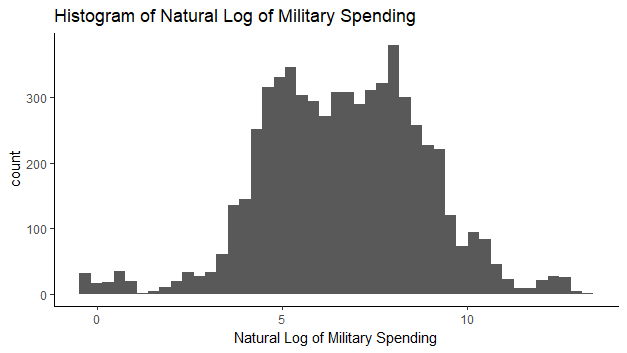
\includegraphics[width=0.95\textwidth]{milex_histogram.png}
	\caption{Distribution of Annual Military Spending by all States: 1950-2001}
	\label{fig:milex_histogram}
\end{figure}

Given all of these concerns, the best model of the arms alliances tradeoff is the work of \citet{DigiuseppePoast2016}, who find that substitution of alliances for arms is conditional on the credibility of the alliance. They argue that that democracies make more credible commitments, and estimate regression models of the association between defense pacts with a democracy and the natural log of military spending, using a lagged dependent variable to account for autocorrelation. All told, the research design in this paper is a marked improvement over prior work.\footnote{While their regression estimator does not account for heavy tails in the dependent variable, the results are robust to using a robust regression estimator.} 

The major shortcoming of DiGiuseppe and Poast's research design is a mismatch between the theory and empirical test. Their theory emphasizes differences in alliances, but then examines differences between states. The binary independent variable captures the presence of a defense pact with a democracy, and coupled with a control for defense pacts with non-democracies, they compare states that have a defense pact with a democracy to states with no defense pacts. DiGiusseppe and Poast's research design is the standard approach in general studies of how alliance membership impacts military spending, which provides minimal detail about differences between alliances.

Unlike general research designs, models of specific alliance dynamics can include more detail about treaty and its members. In these studies, researchers leverage case-specific knowledge to identify critical contextual factors, but focusing on a few alliances limits their generalizability. \citet{PluemperNeumayer2015}'s quasi-spatial model of how NATO members respond to US and Soviet spending is the best evidence of free-riding by NATO members. \citet{Sorokin1994} takes a similar approach to estimating the responses of four states to the military spending of a key ally with a two-stage least squares GLS estimator.

Estimating how alliance membership affects domestic military spending will require researchers to combine the scope of general studies with greater detail about each alliance. Otherwise, differences between alliances will generate omitted variable bias. Although there are few reliable models of how alliance membership affects domestic arms, there are few models of the relationship between the cost of arms and alliance formation. 

\subsection*{Arms Costs and Alliance Formation}

Only two studies consider the other side of the arms-alliances tradeoff--- how the opportunity costs of military spending affect alliance formation. \citet{Kimball2010, AllenDigiuseppe2013} both use panel data, and expect that states with high social demand or costs of sovereign borrowing, will be more likely to form alliances. While these models find the expected positive correlation between the key independent variable and a binary indicator of whether a state joined an alliance in a given year, neither model fits the data well.\footnote{Fit depends on the ability of the model to correctly predict the depdendent variable. Allen and DiGiuseppe's model fits better than Kimball's model.} 

Both models assign low predicted probabilities of alliance formation to observations where formation occurred, as shown by the separation plots in \autoref{fig:formation sep_plot}. Poor model fit casts doubt on the validity of inferences about the covariates \citep{Montgomeryetal2012, Muchlinskietal2015}. Even in state-year panel data, alliance formation is rare, making it more difficult to predict.\footnote{Only 4\% of Kimball's observations and 7\% of Allen and DiGiuseppe's observations see alliance formation.} 

\begin{figure}[htbp]
	\centering
		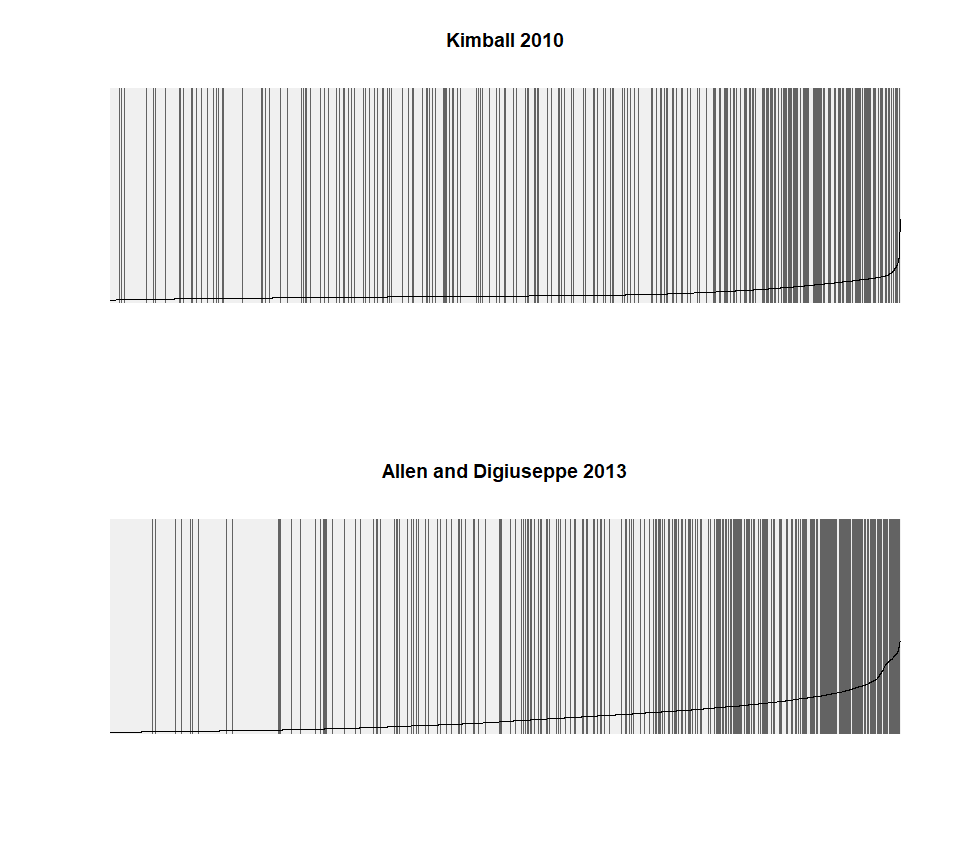
\includegraphics[width=0.90\textwidth]{formation sep_plot.png}
	\caption{Separation plot of primary models from Kimball 2010 and Allen and DiGiuseppe 2013. A separation plot summarizes model fit by ordering observations according to the predicted probability assigned by the model. Dark lines mark observations where the observed value of the dependent variable is one. Better fitting models assign higher predicted probabilities to those observations, which will be reflected by clustering on the right-hand side of the plot. Greater dispersion of the dark lines indicates that the model does a poor job predicting the outcome of interest.}
	\label{fig:formation sep_plot}
\end{figure}

Besides poor model fit, these two research designs indirectly test the logic of substitution. The key independent variable differentiates between states with high opportunity costs of military spending. But the nature of military spending is shifting over time due to increases in the price and complexity of conventional weapons \citep{Bitzinger2003}. Therefore, the marginal utility of a dollar of military spending is not constant over time. Instead, one dollar purchases smaller quantities of military capability.
  
Using panel data with a binary indicator of whether a state formed an alliance in a particular year ignores heterogeneity among alliances. Alliances make different promises, and provide different amounts of capability to support those promises. A defense pact with the United States provides more security than a neutrality pact with Senegal, for instance. The consequential choice of alliance types and partners is neglected by these theories and research designs.  


\subsection*{Overall Empirical Assessment}

If theory testing depends on the accumulation of evidence, we have accumulated little reliable evidence. What we know about the arms-alliance tradeoff depends on two general and three alliance-specific studies. The other 21 research designs are narrow, flawed, or both.  

The core empirical challenge is that the arms-alliances tradeoff contains two distinct levels of analysis. International organizations such as alliances are a separate level of analysis from states \citep{Mattes2012, Chibaetal2015}. Because their outcome of interest is usually at the state level, scholars have relied on crude summaries of the overall alliance portfolio, or only estimated the impact of a few alliances. State-level dummy indicators of alliance membership are the most common independent variable, but this measurement creates substantial problems. 

Using state-level dummy variables in general models restricts the ability of researchers to account for other differences in alliances. Because they average out between-alliance variation, state-level membership proxies remove critical details. For instance, democracies tend to form more limited alliance commitments \citep{Chibaetal2015}, so democratic membership and conditionality are correlated. Other factors such as superpower membership, institutionalization, military aid are also correlated with key alliance conditions. Currently, these alliance characteristics are omitted variables, which could affect our estimates of how alliance membership affects military spending. 

Empirical work on the arms-alliances tradeoff faces similar challenges to other work on the consequences of membership in international organizations. Selection bias is a ubiquitous concern in that literature \citep{Chaudoinetal2016}, but is completely neglected in past research designs. And while theory acknowledges simultaneity between arms and alliances, only one paper (\citet{DigiuseppePoast2016}) uses a simultaneous model. As with theories of the arms-allies tradeoff, there is ample need for improvement in research design.


\section*{Conclusions}

Given theory and empirical evidence, what can we conclude about our understanding of the arms-alliances tradeoff? First, the association between arms and alliances is probably conditional. Research designs must reflect this, and carefully consider the problems inherent in moving between different levels of analysis. 

% abandon free-riding, focus on expenditures-alliance connection, not defense burden

% Reliability and compliance \citep{BerkemeierFuhrmann2018}

% Role of alliance spending/operationalization of membership. Combining detail- alliance spec estimates and general relationships

% Can also consider implications of costs in forming alliances for arms- no one has really done that yet, and it is the inverse of the substitution logic. 



\bibliography{C:/Users/jkalley14/Dropbox/Research/MasterBibliography}  
%\bibliography{C:/Users/Josh/Dropbox/Research/MasterBibliography} 





\end{document}